\section{Related Work: Helping Novices Use Software}
The literature offers several strategies for helping novices effectively use software: some focus on high-level tasks, others on lower-level tool use. \autoref{fig:discoveryspace_ds} describes how our approach relates to this prior work. 

\begin{figure}
\centering
  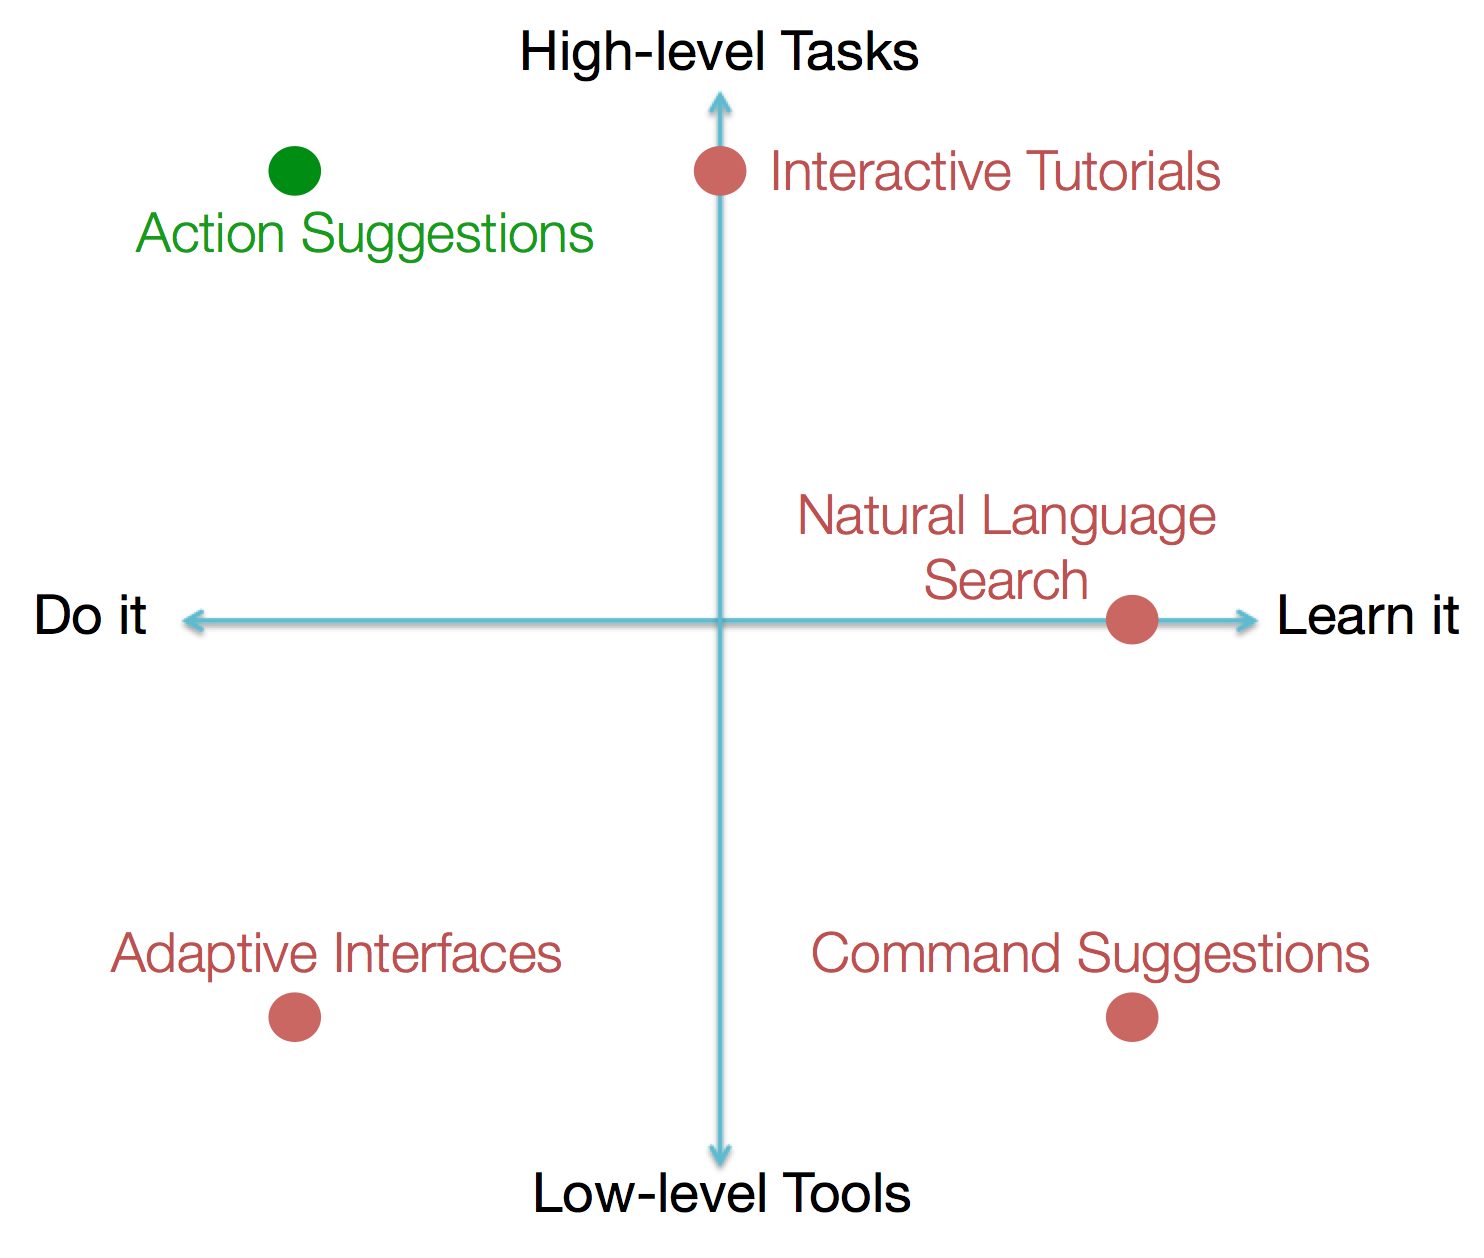
\includegraphics[width=0.6\textwidth]{discoveryspace/figures/designspace.png}
  \caption{Two dimensions along which interventions to help novices can vary. \textit{X-axis}: the goal of the user (whether they want to get things done quickly, or learn the application and its tools). \textit{Y-axis}: the approach to assisting the user (providing high-level tasks or low-level tools).}~\label{fig:discoveryspace_ds}
\end{figure}

\subsection{Interactive Tutorials Provide Step-by-step Guidance}
Online tutorials are a popular resource for users of complex software. However, they present difficulties such as switching back and forth between the browser and the application, and mapping screenshots or videos of the application to the user's own version \cite{Kelleher2005, Pongnumkul2011}. Interactive tutorials address these challenges by guiding users step-by-step through hands-on example tasks inside the target application \cite{Kelleher2005, Lafreniere2014a, Pongnumkul2011}. Such tutorials can even be generated automatically as a user demonstrates them \cite{Grabler2009}. However, there are still far more user goals than authored tutorials, and automatically making static tutorials interactive remains a challenge \cite{Fourney2014Mining, Laput2012}. In addition, users must translate between their own goals and the available tutorials.

Tutorials teach users to use applications step-by-step. Other systems focus on speeding up holistic tasks rather than teaching individual steps. For example, TappCloud introduced ``semi-automated'' tutorials that can be applied in one step, like macros, but also allow for the user to interact with each step if desired \cite{Laput2012}. However, TappCloud users do not interact directly with the application's tools, but instead with visual previews of different parameter settings. Discovery\-Space also focuses on smoothing the execution process rather than helping users learn the application.

\subsection{Adaptively Disclosing Interface Functionality}
Adaptive interfaces initially provide a simplified interface and progressively disclose additional features either automatically \cite{Gajos2006, McGrenere2002, Paymans2004}, or by allowing users to move between predefined interface stages \cite{Carroll1984, Leung2010, McGrenere2002, Shneiderman2000}. Adaptive interfaces are most successful when they are controllable, predictable, efficient, and promote feature discovery \cite{MM-gi2000, Shneiderman2002a}. However, achieving all of these is a well-recognized challenge \cite{Findlater2010, McGrenere2002}. Interfaces that disclose or move features automatically based on user behaviour (\textit{e.g.}, adaptive toolbars in Microsoft Word \cite{Gajos2006}) can improve efficiency, but often feel unpredictable, uncontrollable, and distracting \cite{Gajos2006, Paymans2004, Shneiderman2002a}.

Photoshop Elements is an example of an interface with predefined stages: quick, guided and expert. Users can choose a mode appropriate for their task and skill level, such as quick mode for easily accomplishing basic edits. However, because each mode is associated with a different level of complexity, the interface layout and grouping of tools differs between the modes, making it difficult to transition from one to another.

Adaptive interfaces have mainly focused on task completion efficiency as the performance metric \cite{Gajos2006, Leung2010}. However, for open-ended creative tasks, speed is often less important than discoverability and final quality. Progressive disclosure impedes discoverability by hiding interface elements \cite{Findlater2010}. Discovery\-Space addresses discoverability by suggesting actions users may not have known to be possible.

\subsection{Command Suggestions and Previews}
Most software users are only aware of a small percentage of software features \cite{MM-gi2000}; there may be potential results they could achieve but do not think to try. CommunityCommands introduced the idea that recommending commands to users can improve an application's discoverability \cite{Li2011, Matejka2009}. It uses collaborative filtering to suggest AutoCAD commands that are unknown to the current user but frequently used by others in tandem with the current user's frequent commands. Though command recommendations improve discoverability of new features \cite{Li2011}, suggesting tool-level commands still requires the user to compose and apply them. Inspired by this, Discovery\-Space uses suggestions to promote exploration and discovery, but in the form of task-level actions rather than tool-level commands. 

Previewing results helps users predict what a command will do without having to execute it first. Side Views demonstrated that previews are especially valuable when shown as multiples with different parameter settings \cite{Terry2002}. Building on this, suggesting and previewing alternative courses of action provides users with ideas they may not have considered, speeds the iterative design loop, and shows the contextual effects of changes. Inspired by DesignScape's suggestion interface for graphic design layouts \cite{ODonovan2015}, Discovery\-Space provides both minor (refinement) and major (radical) suggestions.

Popular recommendation algorithms, like collaborative and content-based filtering \cite{Pazzani2007}, rely on users' behaviour and preferences as input. For suggestions within a user interface, the user often begins with a document, 3D model, or image. Suggestions should be content-dependent, since different documents will benefit from different types of operations. For example, DesignScape generates layout suggestions by altering existing elements in the document \cite{ODonovan2015}. Since visual editing operations can have vastly different outcomes on different images \cite{Berthouzoz2011}, it is important to suggest effects that make sense for the content in question. Our algorithm therefore takes into account the content of the image to produce relevant suggestions.

\subsection{Natural Language Search}
To help users find functionality, applications like CommandSpace integrate search directly into the interface \cite{Adar2014}. Natural language search reduces the gap between user language and application language \cite{Adar2014}. Inspired by this work, Discovery\-Space includes search functionality in addition to automatic suggestions. Discovery\-Space also provides simple faceted browsing, the ability to refine a collection based on metadata characteristics \cite{Koren2008}. Facets are especially beneficial for ``exploratory searchers'' who tend to have only a partial idea of what they are looking for \cite{Hearst2006}. Faceted search and browsing were designed for information retrieval tasks; Discovery\-Space extends this underlying idea to executable \textit{actions}.
